\documentclass[11pt,a4paper,twocolumn]{jsarticle}

% documentclassもここに記述するとエラーになる
\usepackage[dvipdfmx]{xcolor} %同上
\usepackage[dvipdfmx]{graphicx} %画像の貼り込みと文字列の変形
% \usepackage{xcolor} %ソースコードの色付け
\usepackage[compatibility=false]{caption} % subcaptionとの競合を避ける
\usepackage{subcaption} % 図のサブキャプションの文字サイズを指定
\usepackage{fancyvrb}

\usepackage{pifont} %テキスト用フォント以外の”特殊な記号を集めたフォント”
\usepackage{bm} %太字の斜体(ボールドイタリック)でベクトルを表現する
\usepackage{bmpsize} %外部プログラムを使用せずにJPEG,PNG,BMPのサイズを計算
\usepackage{amsmath} %数式の記述を容易にし,数式出力の品質を向上させる
\usepackage{amssymb} %同上
\usepackage{comment} %複数行コメントを使うためのパッケージ
\usepackage{here} %図表の配置で[H]を使えるようにする
\usepackage{booktabs} %文中に図を描く
\usepackage{multirow} %同上
\usepackage{setspace} %文書内の行間隔を設定する
\usepackage{siunitx} %国際単位系を簡単に書けるようにする
\usepackage{geometry} %余白の指定
\usepackage{layout} %余白設定を可視化する
\usepackage{ascmac}
\usepackage{paralist} %箇条書きをするのに必要
\usepackage{autobreak} %数式の自動改行
\usepackage{wrapfig}
\usepackage{titlesec}
\usepackage{listings,jlisting} %日本語のコメントアウトをする場合jvlisting(もしくはjlisting)が必要/jlistingのほうがよい
\usepackage{multicol} %文章レイアウトを分割するパッケージ
\usepackage{ulem} %下線を引く

\usepackage{booktabs}  % 表の罫線を太くする
% \usepackage{textcomp}
% \usepackage{tikz}
\usepackage{verbatim}
\usepackage{titlesec} %タイトルの文字サイズを変更する
\usepackage{circuitikz} % 回路図用パッケージ
\usetikzlibrary{circuits.logic.US}
%ここからソースコードの表示に関する設定
\usepackage{mdframed} %文章囲むフレームを作成

\lstset{
    basicstyle=\ttfamily\small,
    keywordstyle=\color{blue}\bfseries,
    commentstyle=\color{darkgray}\itshape,
    stringstyle=\color{red},
    numbers=left,
    numberstyle=\tiny\color{gray},
    stepnumber=1,
    numbersep=5pt,
    backgroundcolor=\color{white},
    frame=single,
    tabsize=4,
    captionpos=b,
    breaklines=true,
    breakatwhitespace=false,
    showspaces=false,
    showstringspaces=false,
    showtabs=false,
    morekeywords={},
    deletekeywords={},
    morecomment=[l]{//},
    morecomment=[s]{/*}{*/},
    morestring=[b]",
    morestring=[b]',
    escapeinside={(*@}{@*)}
}

\lstdefinestyle{pythonstyle}{
    language=Python,
    morekeywords={self, as, with},
    backgroundcolor={\color{white}},
    keywordstyle=\color{blue},
    commentstyle=\color{green},
    stringstyle=\color{red}
}

\newcommand{\fref}[1]{図\ref{#1}} %\fref{fig:}コマンドで"図1"などと表示
\newcommand{\tref}[1]{表\ref{#1}} %\tref{tb:}コマンドで"表1"などと表示
\newcommand{\eref}[1]{式(\ref{#1})} %\eref{eq:}コマンドで"式(1)"などと表示
\newcommand{\lref}[1]{ソースコード\ref{#1}} %\lref{lst:}コマンドで"ソースコード1"などと表示
\newcommand{\sref}[1]{\ref{#1}節} %\sref{}コマンドで"2.1節,2.1.1節"などと表示
\newcommand{\cref}[1]{\ref{#1}章} %\cref{chp:}コマンドで"2章"などと表示
\newcommand{\ShowPython}[1]{%
  \noindent
  \textbf{#1:}
  \lstinputlisting[style=pythonstyle, caption=#1, label=lst:#1]{#1}
  \textbf{Execution Result of #1:}
  \immediate\write18{python #1 > #1.out}%
  \VerbatimInput{#1.out}%
}

\renewcommand{\lstlistingname}{ソースコード}

\titleformat{\section}{\large\bfseries}{\thesection 章}{1em}{}

\geometry{left=10mm,right=10mm,top=10mm,bottom=15mm} %用紙の余白の指定

\def\sec#1{\section{#1}}
\def\ssec#1{\subsection{#1}}
\def\sssec#1{\subsubsection{#1}}

\setlength{\columnsep}{20pt}    % カラム間の間隔を調整
\setlength{\columnseprule}{0.2pt}  % 仕切り線の太さを0.5ptに設定

\begin{document}
    \section{Python入門}
\subsection{Pythonとは}

\subsection{Pythonのインストール}

\subsection{Pythonインタプリタ}

\subsection{Pythonスクリプトファイル}
\subsubsection{ファイルに保存}

\subsubsection{クラス}
\lref{lst:1_Man}にクラスを実装する例を示します。
ここでは、Manという新しいクラスを定義しています。上の例では、
このManというクラスから、mというインスタンス(オブジェクト)を生成します。
Manクラスのコンストラクタ(初期化メソッド)は、nameという引数を取り、その引数でインスタンス変数であるself.nameを初期化します。\textbf{インスタンス変数}とは、個々のインスタンスに格納される変数のことです。Pythonでは、self.nameのように、selfの後に属性名を書くことでインスタンス変数の作成およびアクセスができます。

\subsection{Numpy}

\subsection{Matplotlib}

\subsection{まとめ}

\subsection{ソースコード}
1章のソースコードを以下に示します。

\ShowPython{Man.py}
    \section{パーセプトロン}
\subsection{パーセプトロンとは}
パーセプトロンとは,複数の信号を入力として受けとり,1つの信号を出力する.ここでいう「信号」とは,電流や川のような「流れ」をもつものをイメージするとよいでしょう.電流が同線を流れ,電子を先に送り出すように,パーセプトロンの信号も流れを作り,情報を先へと伝達していきます.たあし,実際の電流とは違い,パーセプトロンの信号は「流す/流さない(1か0)」の二値の値です.本書では,0を「信号を流さない」1を「信号を流す」に対応させて記述します.
さて、\fref{fig:perceptron2}には、2つの信号を入力として受け取るパーセプトロンの例を示しています。$x_1$、$x_2$は入力信号、$y$は出力信号、$w_1$、$w_2$は重みを表します。図の〇は「ニューロン」や「ノード」と呼ばれます。入力信号は、ニューロンに送られる際に、それぞれに固有の重みが乗算されます。ニューロンでは、送られてきた信号の総和が計算され、その総和がある程度限界値を超えた場合にのみ1を出力します。これを「ニューロンが発火する」と表現することもあります。ここでは、その限界値を\textbf{閾値}と呼び、$\theta$という記号で表すことにします。以下にパーセプトロンの動作原理を示します.

\begin{figure}[h]
  \vspace{0mm}
  \begin{center}
    \hspace{0mm}
    \centering
    \includegraphics[width=30mm]{Ch2/peceptron2.png} \
    \vspace{0mm}
    \caption{2入力のパーセプトロン.}
    \label{fig:perceptron2}
  \end{center}
\end{figure}


\begin{equation}
    y = \left\{
\begin{array}{ll}
0 & (b + \omega_1 x_1 + \omega_2 x_2 \le 0)\\
1 & (b + \omega_1 x_1 + \omega_2 x_2 > 0)
\end{array}
    \right.
\end{equation}

\subsection{単純な論理回路}
\subsubsection{ANDゲート}
ANDゲートの真理値表を,\tref{tab:2_AND}に示す.
\begin{table}[htb]
    \centering
    \begin{tabular}{ccc}
        $x_1$ & $x_2$ & $y$ \\  % 1行目
        \hline
        \hline
        0 & 0 & 0 \\  % 2行目
        \midrule
        1 & 0 & 0 \\  % 3行目
        \midrule  % 太い線
        0 & 1 & 0 \\ 
        \midrule  % 太い線
        1 & 1 & 1 \\
        \end{tabular}
    \caption{ANDゲートの真理値表}
    \label{tab:2_AND}
\end{table}

\subsubsection{NANDゲートとORゲート}
NANDゲートとORゲートの真理値表を\tref{tab:2_NAND},\tref{tab:2_OR}に示す.
\begin{table}[htb]
    \centering
    \begin{tabular}{ccc}
        $x_1$ & $x_2$ & $y$ \\  % 1行目
        \hline
        \hline
        0 & 0 & 1 \\  % 2行目
        \midrule
        1 & 0 & 1 \\  % 3行目
        \midrule  % 太い線
        0 & 1 & 1 \\ 
        \midrule  % 太い線
        1 & 1 & 0 \\
        \end{tabular}
    \caption{NANDゲートの真理値表}
    \label{tab:2_NAND}
\end{table}

\begin{table}[htb]
    \centering
    \begin{tabular}{ccc}
        $x_1$ & $x_2$ & $y$ \\  % 1行目
        \hline
        \hline
        0 & 0 & 0 \\  % 2行目
        \midrule
        1 & 0 & 1 \\  % 3行目
        \midrule  % 太い線
        0 & 1 & 1 \\ 
        \midrule  % 太い線
        1 & 1 & 1 \\
        \end{tabular}
    \caption{ORゲートの真理値表}
    \label{tab:2_OR}
\end{table}

\subsection{パーセプトロンの実装}
\subsubsection{簡単な実装}
ANDゲートの実装を\lref{lst:AndGate.py}に示す.

\subsubsection{重みとバイアスの導入}
\begin{equation}
    y=f(x) = \left\{
\begin{array}{ll}
0 & (\omega_1 x_1 + \omega_2 x_2 \le \theta)\\
1 & (\omega_1 x_1 + \omega_2 x_2 > \theta)
\end{array}
    \right.
\end{equation}

\subsubsection{重みとバイアスによる実装}
NANDゲート,ORゲートの実装を\lref{lst:NandGate.py},\lref{lst:OrGate.py}に示す.
AND,NAND,ORは同じ構造のパーセプトロンであり,違いは重みパラメータの値だけ.

\subsection{パーセプトロンの限界}
これまで見てきたように,パーセプトロンを用いれば,AND,NAND,ORの3つの論理回路を実装することができました.それでは続いてXORゲートについて考えてみたいと思います.

\subsubsection{XORゲート}
XORゲートは排他的論理和とも呼ばれる論理回路です.\tref{tab:2_XOR}に示すように,$x_1$と$x_2$のどちらかが1の時だけ出力が1になります.(「排他的」とは自分以外は拒否することを意味します).さて,このXORゲートをパーセプトロンで実装するには,どのような重みパラメータを設定すればよいでしょうか?
実は,これまで見てきたパーセプトロンでは,このXORゲートを実装することはできません.なぜANDやORは実現できて,XORは実現できないのでしょうか.それを説明するために,ここでは図を用いて説明します.以下の図では,0を〇,1を$\square$で表しています.OR
ゲートを作ろうと思えば,\fref{fig:2_OR_png}を直線によって分ける必要があります.実際,左記の直線は,4つの点を正しく分けることができています.
しかし,\fref{fig:2_XOR_png}を直線によって分けることは,いくら考えてもできないでしょう.実は,一本の直線では,〇と$\square$を分けることができないのです.


\begin{table}[htb]
    \centering
    \begin{tabular}{ccc}
        $x_1$ & $x_2$ & $y$ \\  % 1行目
        \hline
        \hline
        0 & 0 & 0 \\  % 2行目
        \midrule
        1 & 0 & 1 \\  % 3行目
        \midrule  % 太い線
        0 & 1 & 1 \\ 
        \midrule  % 太い線
        1 & 1 & 0 \\
        \end{tabular}
    \caption{XORゲートの真理値表}
    \label{tab:2_XOR}
\end{table}

\begin{figure}[htb]
    \vspace{0mm}
    \begin{center}
      \hspace{0mm}
      \centering
      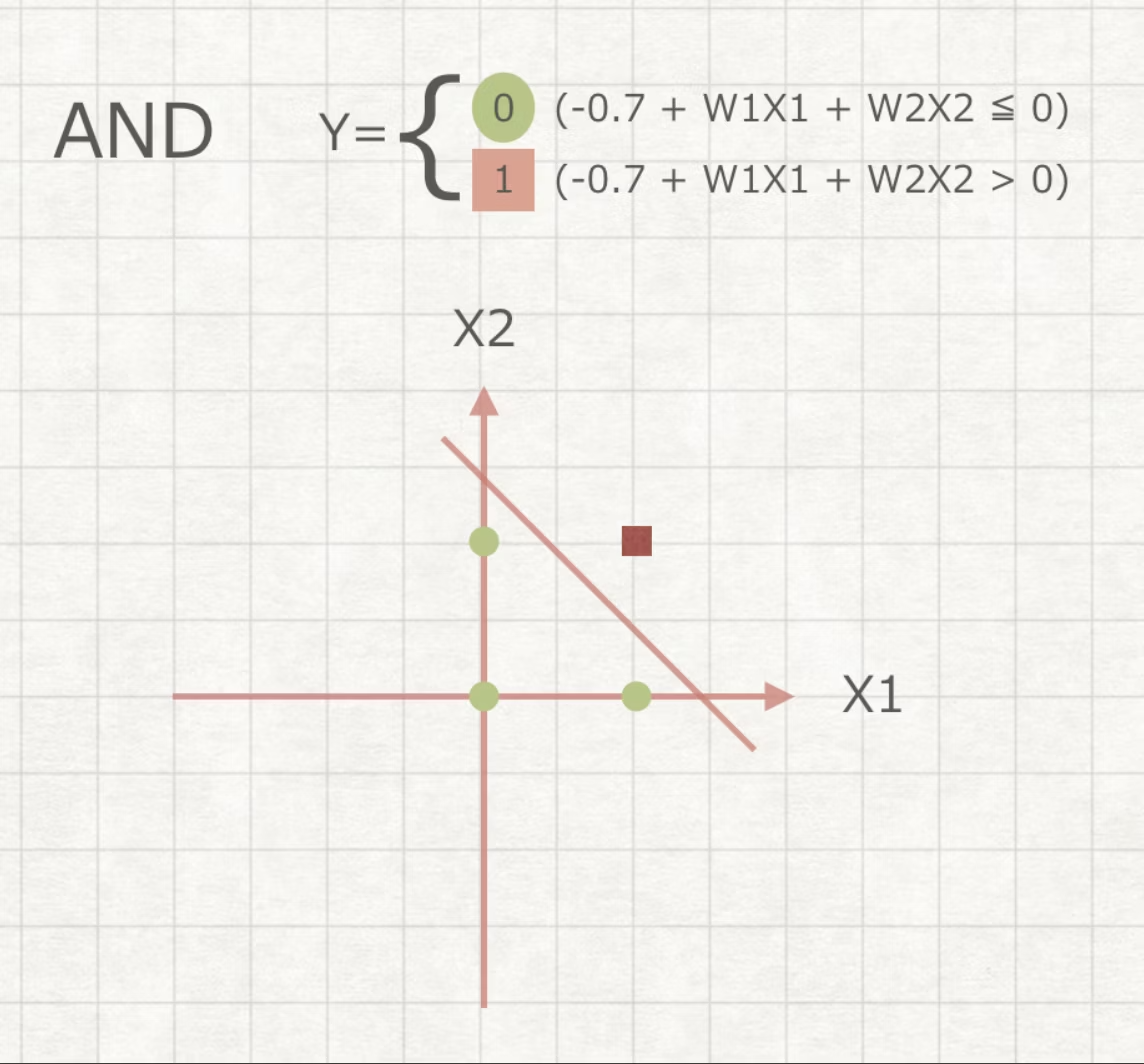
\includegraphics[width=65mm]{../1/Ch2/AND.png} \
      \vspace{0mm}
      \caption{2\_AND\_png}
      \label{fig:2_AND_png}
    \end{center}
  \end{figure}

  \begin{figure}[htb]
    \vspace{0mm}
    \begin{center}
      \hspace{0mm}
      \centering
      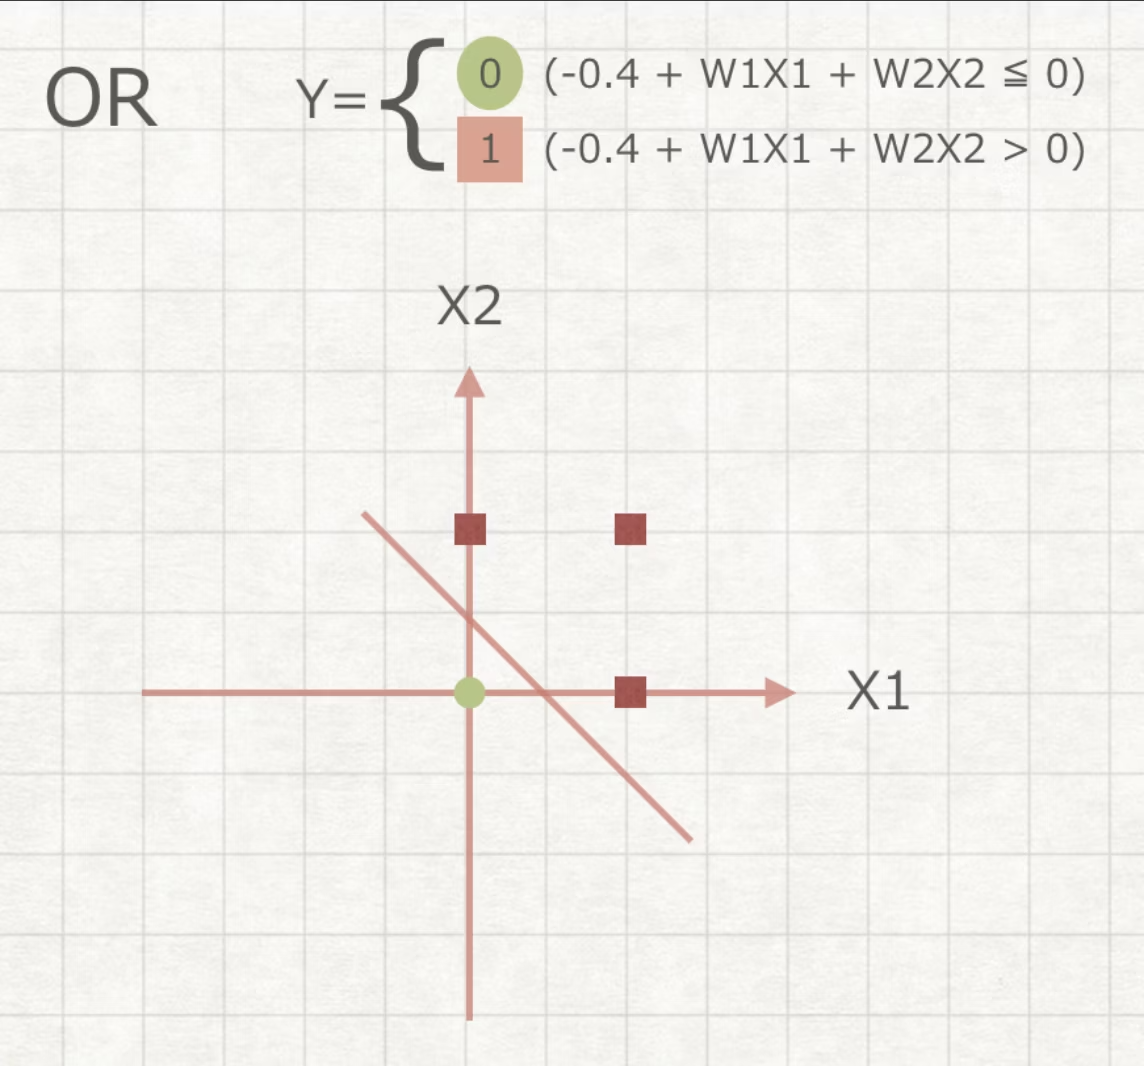
\includegraphics[width=65mm]{../1/Ch2/OR.png} \
      \vspace{0mm}
      \caption{fig:2\_OR\_png}
      \label{fig:2_OR_png}
    \end{center}
  \end{figure}

  \begin{figure}[htb]
    \vspace{0mm}
    \begin{center}
      \hspace{0mm}
      \centering
      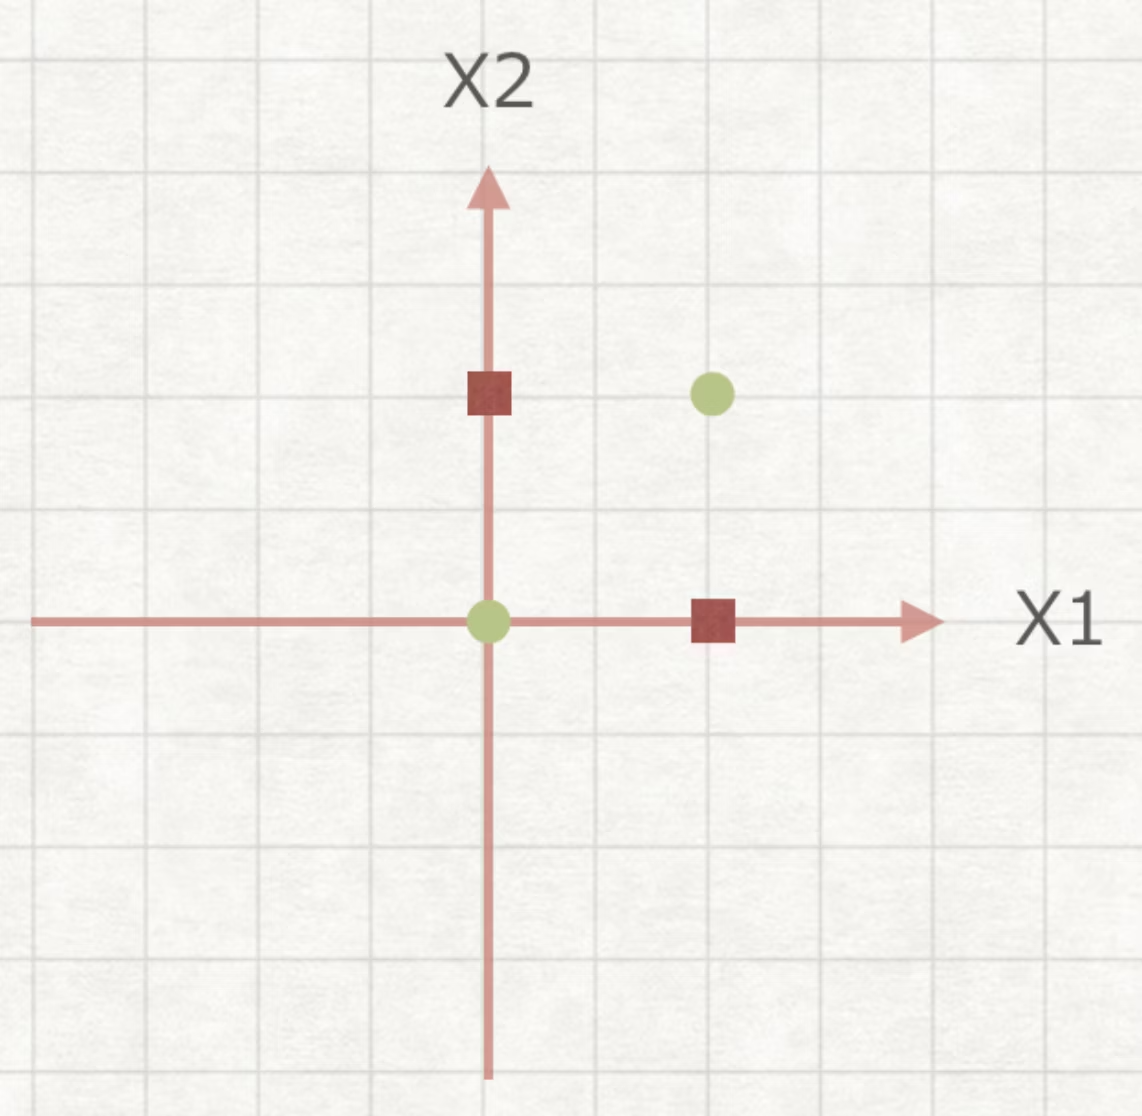
\includegraphics[width=65mm]{../1/Ch2/XOR.png} \
      \vspace{0mm}
      \caption{fig:2\_XOR\_png}
      \label{fig:2_XOR_png}
    \end{center}
  \end{figure}

\subsubsection{線形と非線形}
\fref{fig:2_XOR_png}の〇と$\square$は,一本の直線では分けることができません.しかし,もし"直線"という制約を外すことができたら,〇と$\square$を分けることができます.
\begin{figure}[htb]
    \vspace{0mm}
    \begin{center}
      \hspace{0mm}
      \centering
      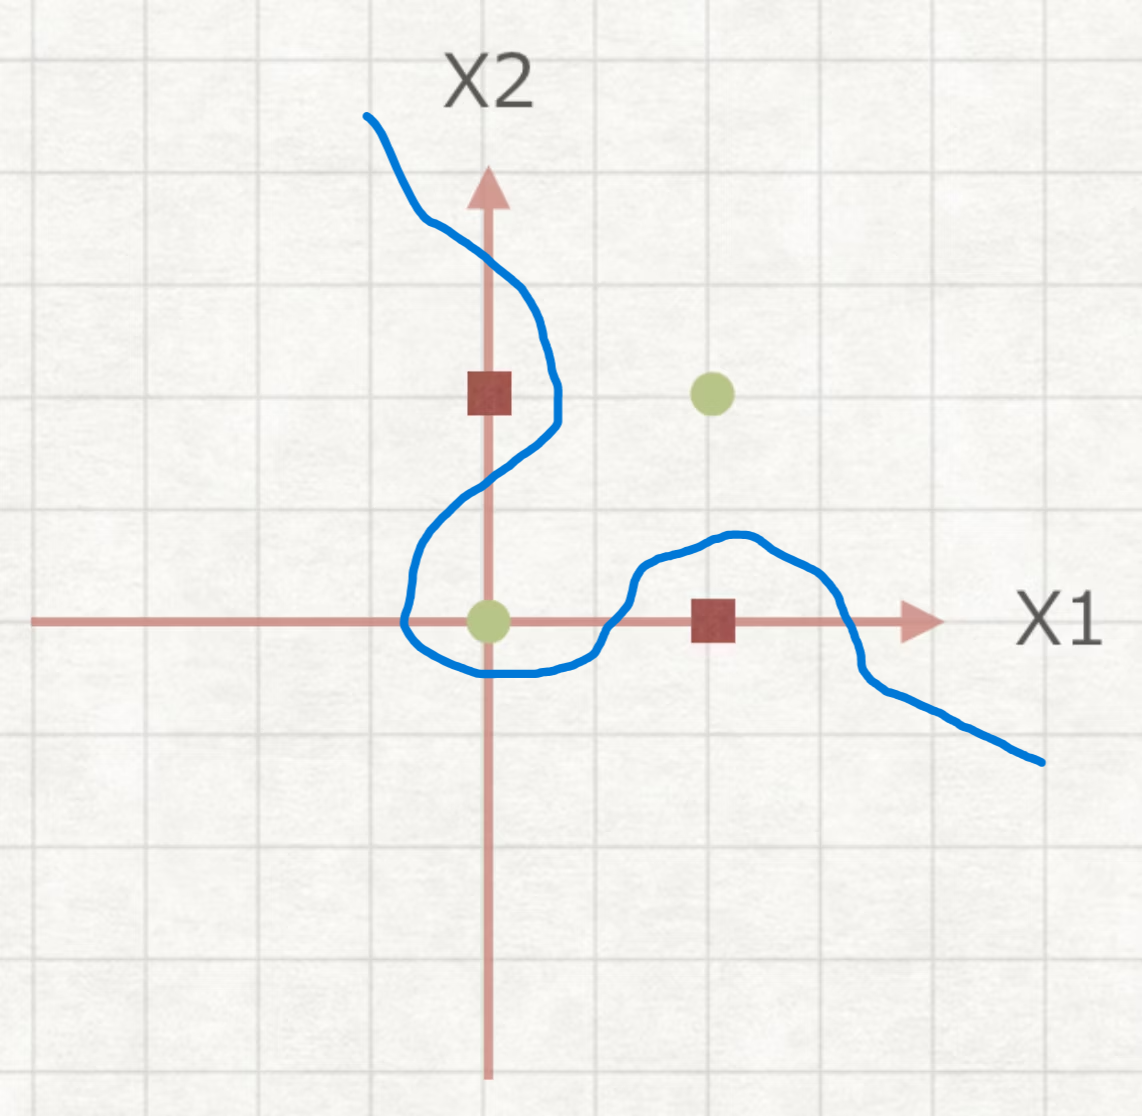
\includegraphics[width=65mm]{../1/Ch2/XOR2.png} \
      \vspace{0mm}
      \caption{fig:2\_XOR2\_png}
      \label{fig:2_XOR2_png}
    \end{center}
  \end{figure}

\subsection{多層パーセプトロン}
残念ながら,パーセプトロンはXORゲートを表現できませんでした.しかし,これは悲しいニュースではありません.実はパーセプトロンの素晴らしさは,"層を重ねる"ことができる点にあります(層を重ねることでXORを表現できるようになるというのが,本筋の筋書です).ここでは「層を重ねる」というのがどう言うことかという説明は後回しにして,XORゲートの問題を別の視点から考えたいと思います.
\subsubsection{既存ゲートの組み合わせ}
XORゲートを作るにはいくつか方法があるが,その一つにAND,NAND,ORゲートを組み合わせる方法がある.XORゲートは教科書の図2-11で実現することができる.\footnote{前節で述べたパーセプトロンの限界は,正確に言うと,「単層のパーセプトロンではXORゲートを表現できない」または「単層のパーセプトロンでは非線形領域は分離できない」ということになります.これから,パーセプトロンを組み合わせることで(層を重ねることで),XORゲートを表現できることを見ていきます.}

\begin{figure}[h]
  \vspace{0mm}
  \begin{center}
    \hspace{0mm}
    \centering
    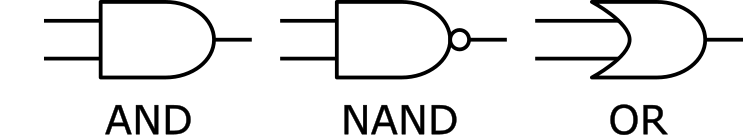
\includegraphics[width=70mm]{Ch2/path13.png} \
    \vspace{0mm}
    \caption{キャプション.}
    \label{fig:ラベル}
  \end{center}
\end{figure}

\begin{figure}[h]
  \vspace{0mm}
  \begin{center}
    \hspace{0mm}
    \centering
    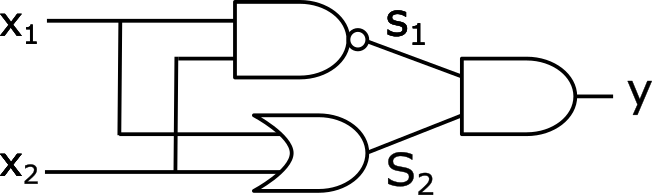
\includegraphics[width=70mm]{Ch2/XOR_AND_NAND_OR.png} \
    \vspace{0mm}
    \caption{キャプション.}
    \label{fig:2_XOR_AND_NAND_OR}
  \end{center}
\end{figure}

\begin{table}[htb]
    \centering
    \begin{tabular}{cc|cc|c}
        $x_1$ & $x_2$ & $s_1$& $s_2$& $y$ \\  % 1行目
        \hline
        \hline
        0 & 0 & 1 & 0 & 0 \\  % 2行目
        \midrule
        1 & 0 & 1& 1& 1 \\  % 3行目
        \midrule  % 太い線
        0 & 1 & 1& 1& 1 \\ 
        \midrule  % 太い線
        1 & 1 & 0& 1& 0 \\
        \end{tabular}
    \caption{XORゲートの真理値表}
    \label{tab:2_XOR_AND_NAND_OR}
\end{table}

\subsubsection{XORゲートの実装}
XORゲートの実装を\lref{lst:XorGate.py}に示す.
XORは、\fref{fig:2_XOR_perceptron}に示すような多層構造のネットワークです。ここでは、一番左の段を第0層、その右の段を第1層、一番右の段を第2層と呼ぶことにします。

さて、\fref{fig:2_XOR_perceptron}のパーセプトロンは、これまで見てきたANDやORが単層のパーセプトロン(\fref{fig:perceptron2})とは異なる形をしています。実際、ANDやORが単層のパーセプトロンであったのに対して、XORは2層のパーセプトロンです。ちなみに、層を複数重ねたパーセプトロンを\textbf{多層パーセプトロン}ということがあります。

\fref{fig:2_XOR_perceptron}に示すような2層のパーセプトロンでは、第0層と第1層のニューロンの間で信号の送受信が行われ、続いて第1層と第2層の間で信号の送受信が行われます。この動作をより詳しく述べると、次のようになります。\footnote{    \fref{fig:2_XOR_perceptron}のパーセプトロンは合計で3層から構成されますが、重みを持つ層は実質2層(第0層と第1層の間、第1層と第2層の間)であるため、
「2層のパーセプトロン」と呼ぶことにします。}

\begin{enumerate}
    \item 第0層の2つのニューロンが入力信号を受け取り、第1層のニューロンへ信号を送る 
    \item 第1層のニューロンが第2層のニューロンへ信号を送り、第2層芽のニューロンは$y$を出力する
\end{enumerate}

\begin{figure}[h]
  \vspace{0mm}
  \begin{center}
    \hspace{0mm}
    \centering
    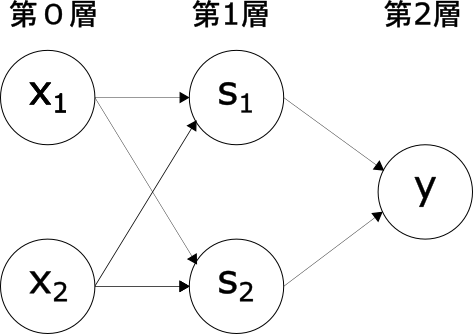
\includegraphics[width=50mm]{Ch2/XOR_perceptron.png} \
    \vspace{0mm}
    \caption{XORのパーセプトロンによる表記.}
    \label{fig:2_XOR_perceptron}
  \end{center}
\end{figure}

\subsection{NANDからコンピュータへ}
コンピュータの内部はとても複雑な処理を行っているように思えますが、実はNANDゲートの組み合わせだけで、コンピュータが行う処理を再現することができるのです。このことは、パーセプトロンでもコンピュータを表現できるということを意味しています。

\subsubsection{まとめ}
\begin{mdframed}[frametitle={本章で学んだこと}]
    \begin{itemize}
        \item パーセプトロンは入出力を備えたアルゴリズムである。ある入力を与えたら、決まった値が出力される。
        \item パーセプトロンでは、「重み」と「バイアス」をパラメータとして設定する。
        \item パーセプトロンを用いれば、AND、OR、NANDゲートなどの論理回路を表現できる。
        \item XORゲートは単層のパーセプトロンでは表現できない。
        \item 2層のパーセプトロンを用いれば、XORゲートを表現できる。
        \item  単層のパーセプトロンは線形領域だけしか分離できないが、多層のパーセプトロンは非線形領域も分離できる。
        \item 多層のパーセプトロンを用いれば、(理論上は)コンピュータが行う処理を再現できる。
    \end{itemize}
\end{mdframed}

\subsection{ソースコード}
2章のソースコードを以下に示します.
\ShowPython{AndGate.py}
\ShowPython{OrGate.py}
\ShowPython{NandGate.py}
\ShowPython{XorGate.py}

    \section{ニューラルネットワーク}
前章ではパーセプトロンについて学びましたが,パーセプトロンについては良いニュースと悪いニュースがありました.良いニュースとは,パーセプトロンの複雑な関数であっても,それを表現できるだけの可能性を秘めているということです.悪いニュースは,重みを設定する作業は,今のところ人の手で行われているということです.

ニューラルネットワークは,先の悪いニュースを解決するためにあります.具体的に言うと,適切な重みパラメータをデータから自動で学習できるというのがニューラルネットワークの重要な性質のひとつです.本章では,ニューラルネットワークの概要を説明し,ニューラルネットワークが識別を行う際の処理に焦点を当てます.そして,次章にて,データから重みパラメータを学習する方法を学びます.
\subsection{パーセプトロンからニューラルネットワークへ}
ニューラルネットワークは,前章で説明したパーセプトロンと共通する点が多くあります.
\subsubsection{ニューラルネットワークの例}
ニューラルネットワークを図で表すと,\fref{fig:3_NeuralNetwork}のようになります.ここで,一番左の列を\textbf{入力層},一番右の列を\textbf{出力層},中間の列を\textbf{中間層}(隠れ層)と呼びます.本書では,入力層から出力層ンい向かって,順に第0層,第1層,第2層と呼ぶことにします.

\begin{figure}[h]
  \vspace{0mm}
  \begin{center}
    \hspace{0mm}
    \centering
    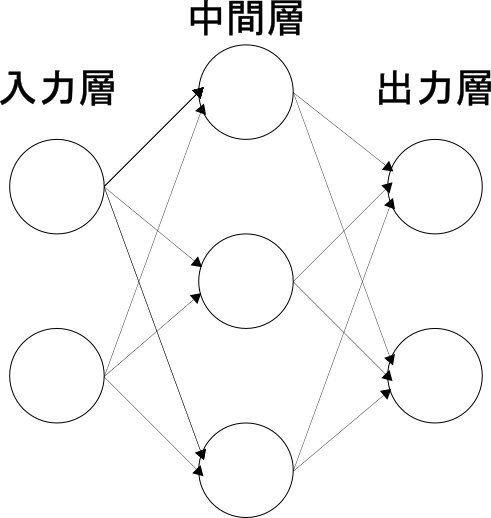
\includegraphics[width=30mm]{Ch3/NeuralNetwork.png} \
    \vspace{0mm}
    \caption{ニューラルネットワークの例}
    \label{fig:3_NeuralNetwork}
  \end{center}
\end{figure}

\subsubsection{パーセプトロンの復習}

\begin{figure}[h]
  \vspace{0mm}
  \begin{center}
    \hspace{0mm}
    \centering
    \includegraphics[width=30mm]{Ch2/peceptron2.png} \
    \vspace{0mm}
    \caption{パーセプトロンの復習}
    \label{fig:3_peceptron2}
  \end{center}
\end{figure}

\fref{fig:3_peceptron2}を数式で表すと\eref{eq:3_peceptron}のようになります.

\begin{equation}
    \label{eq:3_peceptron}
    y = \left\{
\begin{array}{ll}
0 & (b + \omega_1 x_1 + \omega_2 x_2 \le 0)\\
1 & (b + \omega_1 x_1 + \omega_2 x_2 > 0)
\end{array}
    \right.
\end{equation}

$b$を明示したものを\fref{fig:3_vias}に示す.\eref{eq:3_peceptron}をよりシンプルな形に書き換える.

\begin{figure}[h]
  \vspace{0mm}
  \begin{center}
    \hspace{0mm}
    \centering
    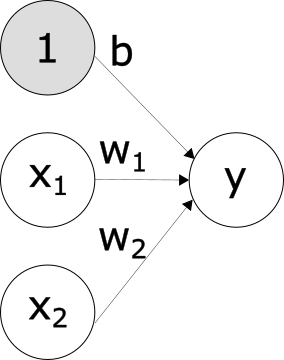
\includegraphics[width=30mm]{Ch3/vias.png} \
    \vspace{0mm}
    \caption{バイアスを明示的に示す}
    \label{fig:3_vias}
  \end{center}
\end{figure}




\eref{eq:3_peceptron_simple}は,入力信号の総和が$h(x)$という関数によって変換され,その変換された値が出力$y$になるということを表しています.そして,\eref{eq:3_step_function}で表された$h(x)$関数は,入力が0を超えたら1を返し,そうでなければ1を返します.そのため,\eref{eq:3_peceptron}と\eref{eq:3_peceptron_simple},\eref{eq:3_step_function}は同じことを行っているのです.

\subsubsection{活性化関数の登場}
**..

\begin{equation}
    \label{eq:3_peceptron_simple2}
a=b+\omega_1 x_1 + \omega_2 x_2
\end{equation}

\begin{equation}
    \label{eq:3_step_function2}
y=h(a)
\end{equation}

\eref{eq:3_peceptron_simple2}では,重み付き入力信号とバイアスの総和を計算し,それを$a$とします.\eref{eq:3_step_function2}では,$a$が$h(x)$で変換され$y$が出力される,という流れになります.

それでは続いて活性化関数について詳しく見ていくことにします.この活性化関数が,パーセプトロンからニューラルネットワークへ進むための懸け橋になります.\footnote{「パーセプトロン」という言葉がさすアルゴリズムは,本書では厳密な統一がされずに使われています.一般的に,「単純パーセプトロン」といえば,それは単層のネットワークで,活性化関数にステップ関数を使用したモデルを指します.「多層パーセプトロン」というと,それはニューラルネットワーク-多層で,シグモイド関数などの滑らかな活性化関数を使用するネットワーク-を指すのが一般的です.
}


\subsection{活性化関数}
「パーセプトロンでは、活性化関数にステップ関数を利用している」ということができる。つまり、活性化関数の候補としてたくさんある関数の中で、パーセプトロンは「ステップ関数」を採用しているのです。活性化関数にステップ関数以外の関数を採用することで、ニューラルネットワークの世界へと進むことができるのです!

\subsubsection{シグモイド関数}
ニューラルネットワークでよく用いられる活性化関数の一つは、\eref{eq:3_sigmoid}で表されるシグモイド関数です.

\begin{equation}
    \label{eq:3_sigmoid}
    h(x) = \frac{1}{1 + \exp(-x)}
\end{equation}

前章で見たパーセプトロンとこれから見ていくニューラルネットワークの主な違いは、この活性化関数だけなのです。

\subsubsection{ステップ関数の実装}
\ShowPython{THstep.py}
\begin{figure}[H]
  \vspace{0mm}
  \begin{center}
    \hspace{0mm}
    \centering
    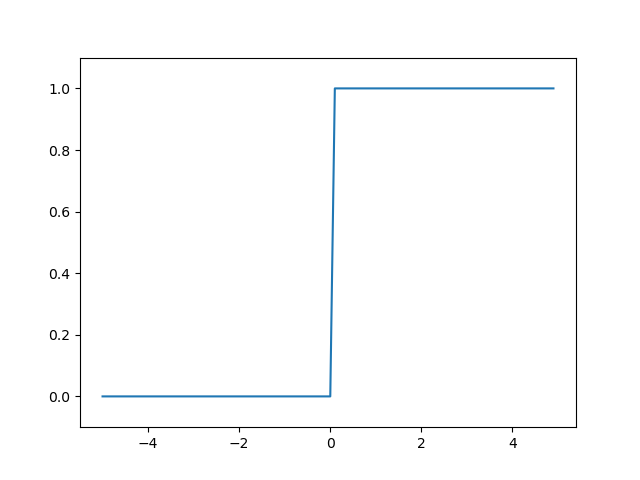
\includegraphics[width=40mm]{Ch3/step.png} \
    \vspace{0mm}
    \caption{ステップ関数のグラフ}
    \label{fig:3_step}
  \end{center}
\end{figure}

\subsubsection{シグモイド関数の実装}
\ShowPython{THsigmoid.py}
\begin{figure}[h]
  \vspace{0mm}
  \begin{center}
    \hspace{0mm}
    \centering
    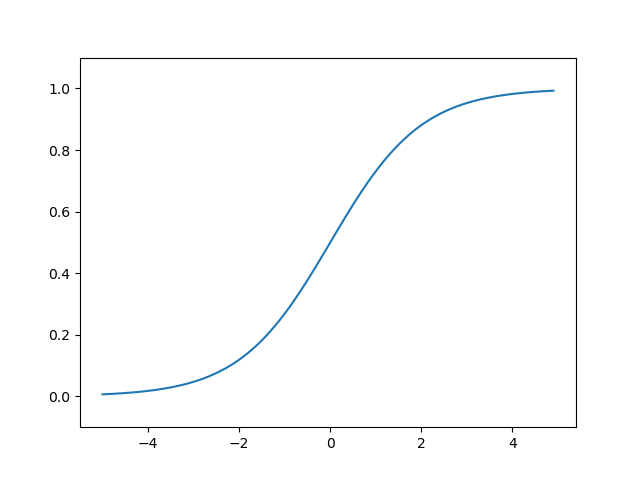
\includegraphics[width=40mm]{Ch3/sigmoid.png} \
    \vspace{0mm}
    \caption{シグモイド関数のグラフ}
    \label{fig:3_sigmoid}
  \end{center}
\end{figure}

\subsubsection{シグモイド関数とステップ関数の比較}
\ShowPython{THstepsigmoid.py}
\begin{figure}[H]
  \vspace{0mm}
  \begin{center}
    \hspace{0mm}
    \centering
    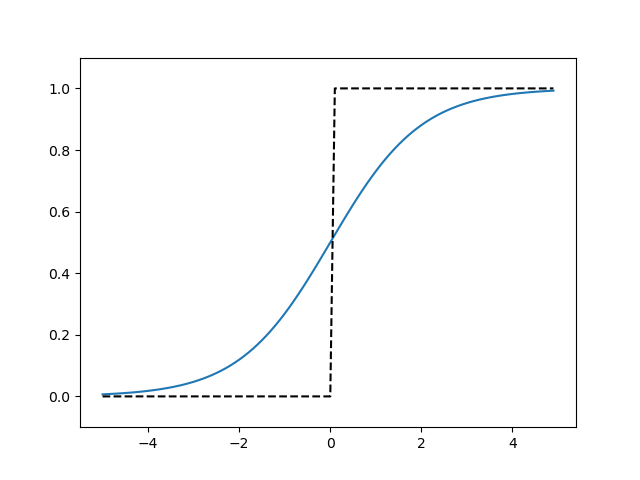
\includegraphics[width=50mm]{Ch3/SigmoidStep.png} \
    \vspace{0mm}
    \caption{ステップ関数とシグモイド関数(破線はステップ関数)}
    \label{fig:3_SigmoidStep}
  \end{center}
\end{figure}

両者とも、入力信号が重要な情報であれば大きな値を出力し、入力信号が重要でなければ小さな値を出力するのです。そして、どんなに入力信号の値が小さくても、またどんなに入力信号の値が大きくても、出力信号の値を0から1の間に押し込めるのも両者の共通点です。

\subsubsection{非線形関数}

\subsubsection{ReLu関数}
これまでに活性化関数としてステップ関数とシグモイド関数を紹介しました。シグモイド関数は、ニューラルネットワークの歴史において、古くから利用されてきました。しかし、最近では\textbf{ReLU関数}(Rectified Linear Unit)という関数が主に用いられます(\fref{fig:3_relu}参照)。

\ShowPython{THrelu.py}
\begin{figure}[h]
  \vspace{0mm}
  \begin{center}
    \hspace{0mm}
    \centering
    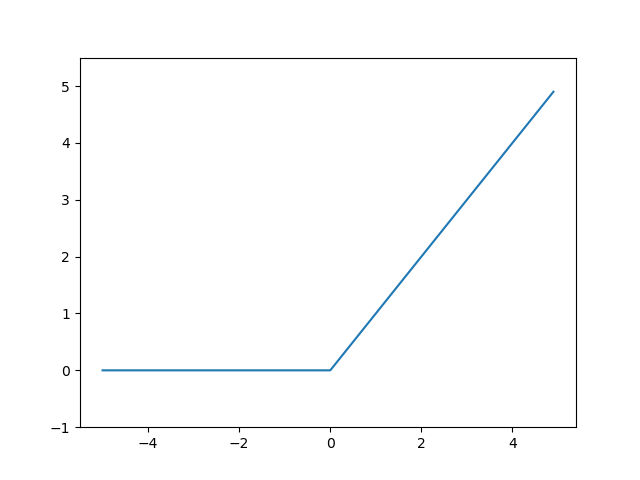
\includegraphics[width=50mm]{Ch3/relu.png} \
    \vspace{0mm}
    \caption{ReLU関数}
    \label{fig:3_relu}
  \end{center}
\end{figure}

ReLU関数を数式で表すと、\eref{eq:3_relu}のようになります。

\begin{equation}
    \label{eq:3_relu}
    h(x) = \left\{
\begin{array}{ll}
x & (x > 0)\\
0 & (x \le 0)
\end{array}
    \right.
\end{equation}

グラフや数式の通り、ReLU関数はとてもシンプルな関数です。そのため、実装もとても容易です。

さて、本章の残りでは、活性化関数にシグモイド関数を使用していきますが、本書の後半では主にReLU関数を使用していきます。

\subsection{多次元配列の計算}
ここではNumpyによる多次元配列の計算について説明し、その後にニューラルネットワークの実装を行っていきます。
\subsubsection{多次元配列}
\subsubsection{行列の積}
\subsubsection{ニューラルネットワークの行列の積}


\end{document}